%================================================
%	PACKAGES AND THEMES
%================================================
\documentclass[t,aspectratio=169,xcolor=dvipsnames]{beamer}
\usetheme{metropolis}
\usecolortheme{metropolis}
\setbeamercolor{background canvas}{bg=white}
\setbeamercolor{frametitle}{bg=black,fg=white}
\usepackage{graphicx} % For images
\usepackage{tikz} % For your diagrams
\usepackage[svgnames,table]{xcolor} % For color options
\usepackage{fontawesome} % For your icons in the outline
\usepackage{natbib} % For your references
\usepackage{colortbl}
\usepackage{xcolor}


%================================================
%	BEGIN DOCUMENT 
%================================================
\begin{document}

%================================================
%	TITLE PAGE
%================================================
\title[short title]{Influences on Soccer Player Value} 
\subtitle{An Analysis of Transfermarkt and Europe's Top 5 Leagues}

\author{Devin Williams}
\institute[OU]{ECON 5253 \\ University of Oklahoma \\}

\date{{April 29th, 2025}}

\begin{frame}[plain]
    \titlepage
\end{frame}

%------------------------------------------------
%	OUTLINE SLIDE
%------------------------------------------------
\begin{frame}[plain]
    \frametitle{Table of Contents} 
    \framesubtitle{~}
\vspace{0.5cm}
    \begin{columns}[T]
        % Left column
        \begin{column}{0.48\textwidth}
            \begin{itemize}
                \item[\faInfoCircle] \textbf{Introduction}
                \begin{itemize}
                    \item Significance of The World's Game
                    \item Operational Definitions
                    \item Margin of Error
                \end{itemize}
                
                \item[\faDatabase] \textbf{Data}
                \begin{itemize}
                    \item TransferMarkt and API
                \end{itemize}
            \end{itemize}
        \end{column}
        
        % Right column
        \begin{column}{0.48\textwidth}
            \begin{itemize}
                \item[\faLineChart] \textbf{Methods}
                \begin{itemize}
                    \item Finding Connections
                    \item Club Categories
                    \item Regression Equations
                \end{itemize}
                \item[\faSearch] \textbf{Findings}
                \begin{itemize}
                    \item Regression Findings
                    \item Peak Age
                \end{itemize}
                \item[\faCheck] \textbf{Conclusion}
            \end{itemize}
        \end{column}
    \end{columns}
\end{frame}
%~~~~~~~~~~~~~~~~~~~~~~~~~~~~~~~~~~~~~~~~~~~~~~~~
\section{Introduction}
%~~~~~~~~~~~~~~~~~~~~~~~~~~~~~~~~~~~~~~~~~~~~~~~~

%------------------------------------------------
%	NEW SLIDE
%------------------------------------------------
%~~~~~~~~~~~~~~~~~~~~~~~~~~~~~~~~~~~~~~~~~~~~~~~~
\subsection{Significance of the World's Game}
%~~~~~~~~~~~~~~~~~~~~~~~~~~~~~~~~~~~~~~~~~~~~~~~~
\begin{frame}
    \frametitle{Significance of the World's Game}
    \vspace{0.5cm} % Add space after the title
    \begin{itemize}
        \item 1.5 Billion people watched the World Cup Final in 2022 \citep{Worldcupratings}. 
        \item Highest paid player in Europe - Robert Lewandowski \citep{Lewandowski}.
        \item Other players worldwide make more, but Europe is the highest level of competition. 
    \end{itemize}
\end{frame}

%~~~~~~~~~~~~~~~~~~~~~~~~~~~~~~~~~~~~~~~~~~~~~~~~
\subsection{Operational Definitions}
%~~~~~~~~~~~~~~~~~~~~~~~~~~~~~~~~~~~~~~~~~~~~~~~~

%------------------------------------------------
%	NEW SLIDE
%------------------------------------------------
\begin{frame}
    \frametitle{Operational Definitions} 
     \begin{itemize}
        \item Transfer/"Sell"
        \item Transfer Value/Market Value
        \item Release Clause
        \item "The Big 5"
        \item Club
        \item Relegation/Promotion
        \item Transfermarkt
    \end{itemize}
\end{frame}
%------------------------------------------------
%	NEW SLIDE
%------------------------------------------------
\begin{frame}
    
    \begin{center}
        \vspace{3cm} % Add some vertical space
        \huge{\textbf{€10,960,000,000}}
        \vspace{2cm} % Add some vertical space
    \end{center}

\end{frame}

%------------------------------------------------
%	NEW SLIDE
%------------------------------------------------
\begin{frame}
    
    \begin{center}
        \vspace{3cm} % Add some vertical space
        \huge{\textbf{Amount spent in JUST 2024 on Player Transfers \citep{TransferSpending}.}}
        \vspace{2cm} % Add some vertical space
    \end{center}

\end{frame}

%~~~~~~~~~~~~~~~~~~~~~~~~~~~~~~~~~~~~~~~~~~~~~~~~
\subsection{Margin of Error}
%~~~~~~~~~~~~~~~~~~~~~~~~~~~~~~~~~~~~~~~~~~~~~~~~

%------------------------------------------------
%	NEW SLIDE
%------------------------------------------------
\begin{frame}
    \frametitle{Margin of Error - Neymar Jr.}
    
    \begin{center}
    \begin{tikzpicture}
        % First image
        \node (img1) {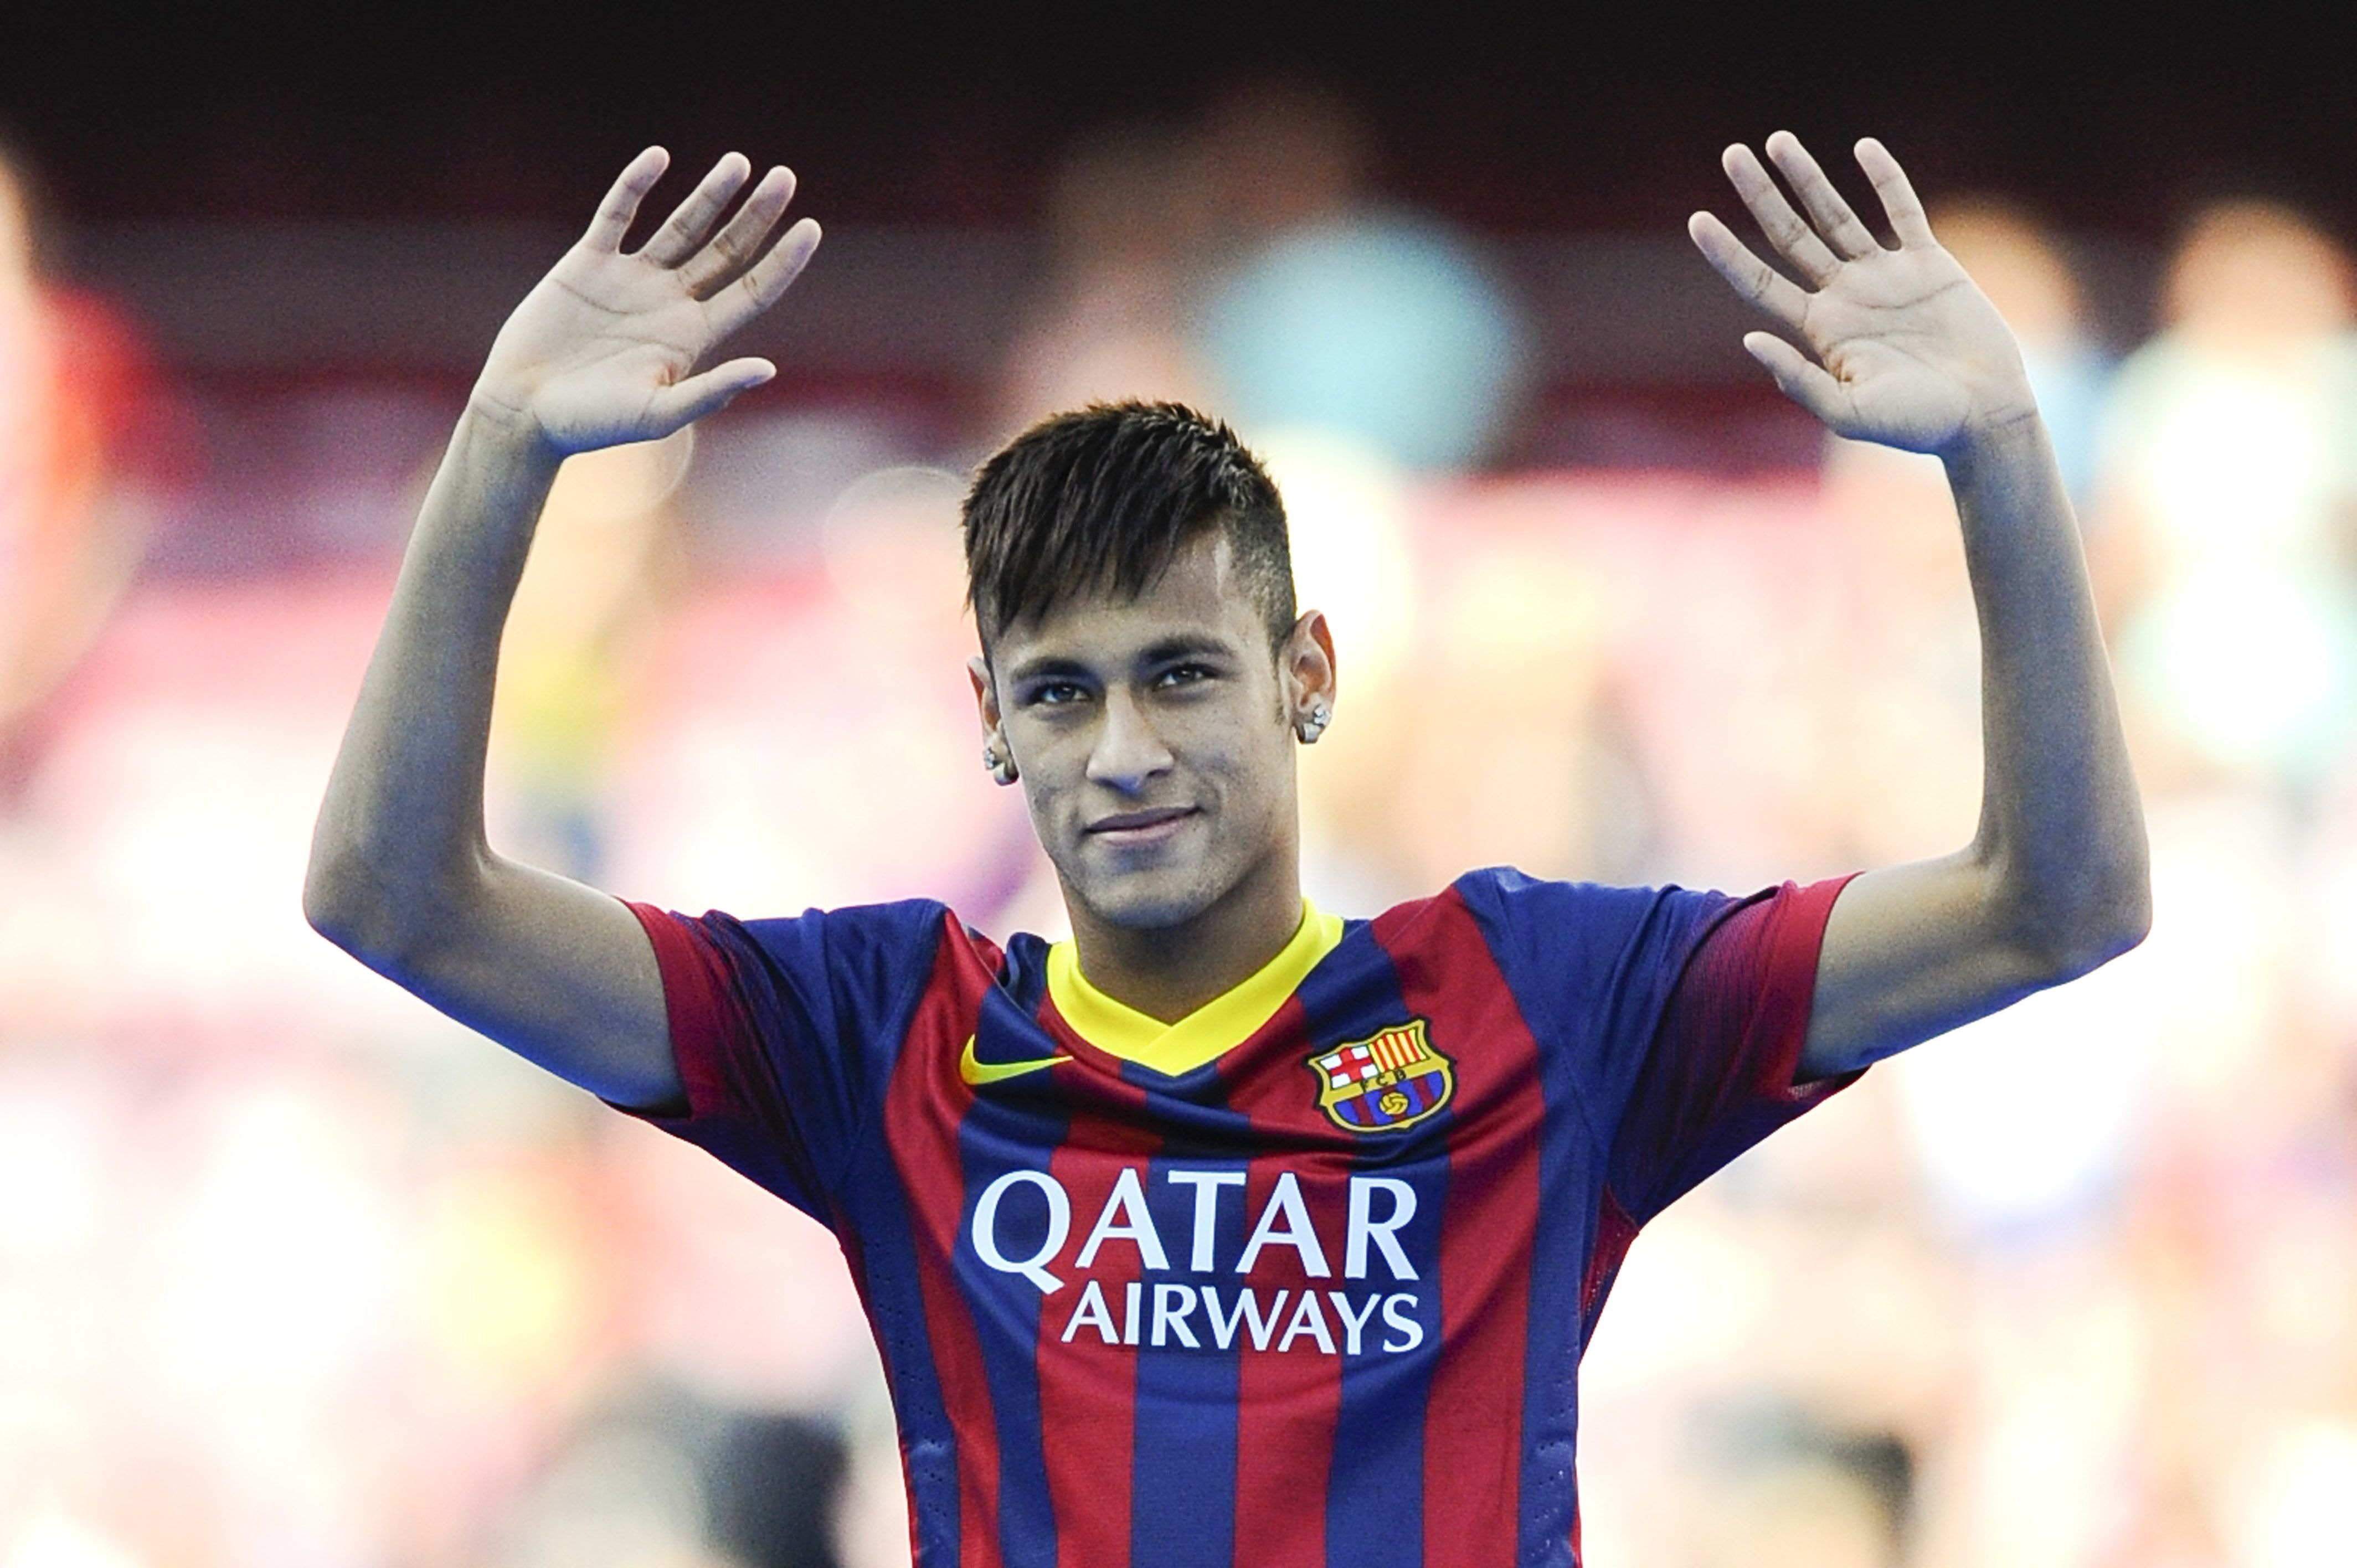
\includegraphics[width=0.3\textwidth]{pictures/NeymarBarca.jpg}};
        
        % Second image with the same size, placed further to the right
        \node (img2) at (8,0) {
\includegraphics[width=0.3\textwidth]{pictures/NeymarPSG.jpg}};
        
        % Draw arrow between images - longer now with more space
        \draw[->, thick] (img1.east) -- (img2.west) 
            node[midway, above] {Market value (100m)} 
            node[midway, below] {True price (222m)};
    \end{tikzpicture}
    \end{center}
    
    \begin{itemize}
        \item A lot of different factors can impact true sale price. 
        \item Transfermarkt can't quantify everything. 
    \end{itemize}
\end{frame}

%------------------------------------------------
%	NEW SLIDE
%------------------------------------------------
\begin{frame}
    \frametitle{Margin of Error - Frankie De Jong}
    
    \begin{center}
    \begin{tikzpicture}
        % First image
        \node (img1) {
\includegraphics[width=0.3\textwidth]{pictures/DejongAjax.jpg}};
        
        % Second image with the same size, placed further to the right
        \node (img2) at (8,0) {
\includegraphics[width=0.3\textwidth]{pictures/de-jong-barca-scaled.jpg}};
        
        % Draw arrow between images - longer now with more space
        \draw[->, thick] (img1.east) -- (img2.west) 
            node[midway, above] {Market value (85m)} 
            node[midway, below] {True price (86m)};
    \end{tikzpicture}
    \end{center}
    
    \begin{itemize}
        \item Many causes, evaluations are close to being accurate selling prices. 
        \item This study looked to understand factors to the website Transfermarkts player evaluations, while evaluating country of origin biases. 
    \end{itemize}
    
\end{frame}

%~~~~~~~~~~~~~~~~~~~~~~~~~~~~~~~~~~~~~~~~~~~~~~~~
\section{Data}
%~~~~~~~~~~~~~~~~~~~~~~~~~~~~~~~~~~~~~~~~~~~~~~~~
%~~~~~~~~~~~~~~~~~~~~~~~~~~~~~~~~~~~~~~~~~~~~~~~~
\subsection{TransferMarkt and API}
%~~~~~~~~~~~~~~~~~~~~~~~~~~~~~~~~~~~~~~~~~~~~~~~~

%------------------------------------------------
%	NEW SLIDE
%------------------------------------------------
\begin{frame}

    \frametitle{Transfermarkt and API} 

     \begin{itemize}
        \item Transfermarkt is a site where people "go to find, and discuss, information about soccer players" \citep{Wisdom_Crowd}.
        \item The website is a leader in player and club evaluations. \citep{Wisdom_Crowd}. 
        \item Absence of a algorithm \citep{Wisdom_Crowd}.
        \item This project utilizes a third-party Github repository that allows access to an unofficial Transfermarkt API \citep{GithubAPI}.
        \item This API was used to download data related to player demographics, club and league information, performance metrics, and current market evaluations. 
    \end{itemize}
\end{frame}

%~~~~~~~~~~~~~~~~~~~~~~~~~~~~~~~~~~~~~~~~~~~~~~~~
\section{Methods}
%~~~~~~~~~~~~~~~~~~~~~~~~~~~~~~~~~~~~~~~~~~~~~~~~
%~~~~~~~~~~~~~~~~~~~~~~~~~~~~~~~~~~~~~~~~~~~~~~~~
\subsection{Finding Connections}
%~~~~~~~~~~~~~~~~~~~~~~~~~~~~~~~~~~~~~~~~~~~~~~~~
%------------------------------------------------
%	NEW SLIDE
%------------------------------------------------
\begin{frame}

    \frametitle{Finding Connections} 

     \begin{itemize}   
        \item Data was collected to understand what impacts market evaluation.
        \item Systematic comparisons were done of market values across continents, performance metrics, positions, and age groups. 
        \item Player's age was squared to evaluate the non-linearity of age in the sample. 
        \item Log-linear regression models were done for each position group. 
    \end{itemize}
    

\end{frame}

%~~~~~~~~~~~~~~~~~~~~~~~~~~~~~~~~~~~~~~~~~~~~~~~~
\subsection{Club Categories}
%~~~~~~~~~~~~~~~~~~~~~~~~~~~~~~~~~~~~~~~~~~~~~~~~
%------------------------------------------------
%	NEW SLIDE
%------------------------------------------------
\begin{frame}

    \frametitle{Club Categories} 

     \begin{itemize}   
        \item Clubs are put into 5 different categories. 
        \item Elite Clubs, Strong Clubs, Mid-Table Clubs, Lower-Tier Clubs, and Other Clubs. 
        \item Teams are split based on Rescaled squad value (40\%), maximum player value(30\%), squad size(20\%), and youthfulness(10\%) of the squad. 
        \item Z-scores used to standardize the average squad value within each league. This is meant to allow fairer comparison across leagues. 
    \end{itemize}
        
    \resizebox{\textwidth}{!}{
    
\begin{tabular}{|l|l|}
\hline
\textbf{Tier} & \textbf{Examples} \\
\hline
\textbf{Tier 1: Elite Clubs} & 

\includegraphics[height=1em]{badges/real_madrid.png}~Real Madrid, 

\includegraphics[height=1em]{badges/barcelona.png}~Barcelona, 

\includegraphics[height=1em]{badges/bayern.png}~Bayern Munich \\
\hline
\textbf{Tier 2: Strong Clubs} & 

\includegraphics[height=1em]{badges/monaco.png}~AS Monaco, 

\includegraphics[height=1em]{badges/newcastle.png}~Newcastle United, 

\includegraphics[height=1em]{badges/atletico.png}~Atletico Madrid \\
\hline
\textbf{Tier 3: Mid-Table Clubs} & 

\includegraphics[height=1em]{badges/aston_villa.png}~Aston Villa, 

\includegraphics[height=1em]{badges/crystal_palace.png}~Crystal Palace, 

\includegraphics[height=1em]{badges/brentford.png}~Brentford FC \\
\hline
\textbf{Tier 4: Lower-Tier Clubs} & 

\includegraphics[height=1em]{badges/girona.png}~Girona FC, 

\includegraphics[height=1em]{badges/leicester.png}~Leicester City, 

\includegraphics[height=1em]{badges/reims.png}~Stade Reims \\
\hline
\textbf{Tier 5: Other Clubs} & 

\includegraphics[height=1em]{badges/betis.png}~Real Betis, 

\includegraphics[height=1em]{badges/nantes.png}~FC Nantes, 

\includegraphics[height=1em]{badges/union_berlin.png}~FC Union Berlin \\
\hline
\end{tabular}
}

\end{frame}

%------------------------------------------------
%	NEW SLIDE
%------------------------------------------------
%~~~~~~~~~~~~~~~~~~~~~~~~~~~~~~~~~~~~~~~~~~~~~~~~
\subsection{Regression Equations}
%~~~~~~~~~~~~~~~~~~~~~~~~~~~~~~~~~~~~~~~~~~~~~~~~
\begin{frame}
    \frametitle{Regression Equations}
    
    \begin{columns}[T]
        \begin{column}{0.58\textwidth}
            \begin{equation}
            \begin{split}
            \ln(MarketValue_i) = & \beta_0 + \beta_1 Continent_i + \beta_2 Age_i \\
                                 & + \beta_3 AgeSquared_i \\
                                 & + \beta_4 Appearances_i \\
                                 & + \beta_5 GoalContributions_i^* \\
                                 & + \beta_6 League_i + \beta_7 ClubTier_i + \varepsilon_i
            \end{split}
            \end{equation}
            \vspace{-0.3cm}
            {\footnotesize $^*$Not included in the goalkeeper model}
        \end{column}
        
        \begin{column}{0.42\textwidth}
            \vspace{0.1cm}
            \footnotesize
            \textbf{Where:}
            \begin{itemize}
                \item $MarketValue_i$ = Value in € (By position)
                \item $Continent_i$ = Origin (ref: Europe)
                \item $Age_i$ = Age in years
                \item $AgeSquared_i$ = Age$^2$
                \item $Appearances_i$ = Games played in last 2 years
                \item $GoalContributions_i$ = Goals+assists in last 2 years
                \item $League_i$ = League (ref: EPL)
                \item $ClubTier_i$ = Club tier (ref: Elite)
                \item $\varepsilon_i$ = Error term
            \end{itemize}
        \end{column}
    \end{columns}
\end{frame}

%~~~~~~~~~~~~~~~~~~~~~~~~~~~~~~~~~~~~~~~~~~~~~~~~
\subsection{Data Exploration}
%~~~~~~~~~~~~~~~~~~~~~~~~~~~~~~~~~~~~~~~~~~~~~~~~
%------------------------------------------------
%	NEW SLIDES
%------------------------------------------------

% Slide 1
\begin{frame}
    \frametitle{Player Distribution by Position Group}
    \begin{figure}
        \centering
        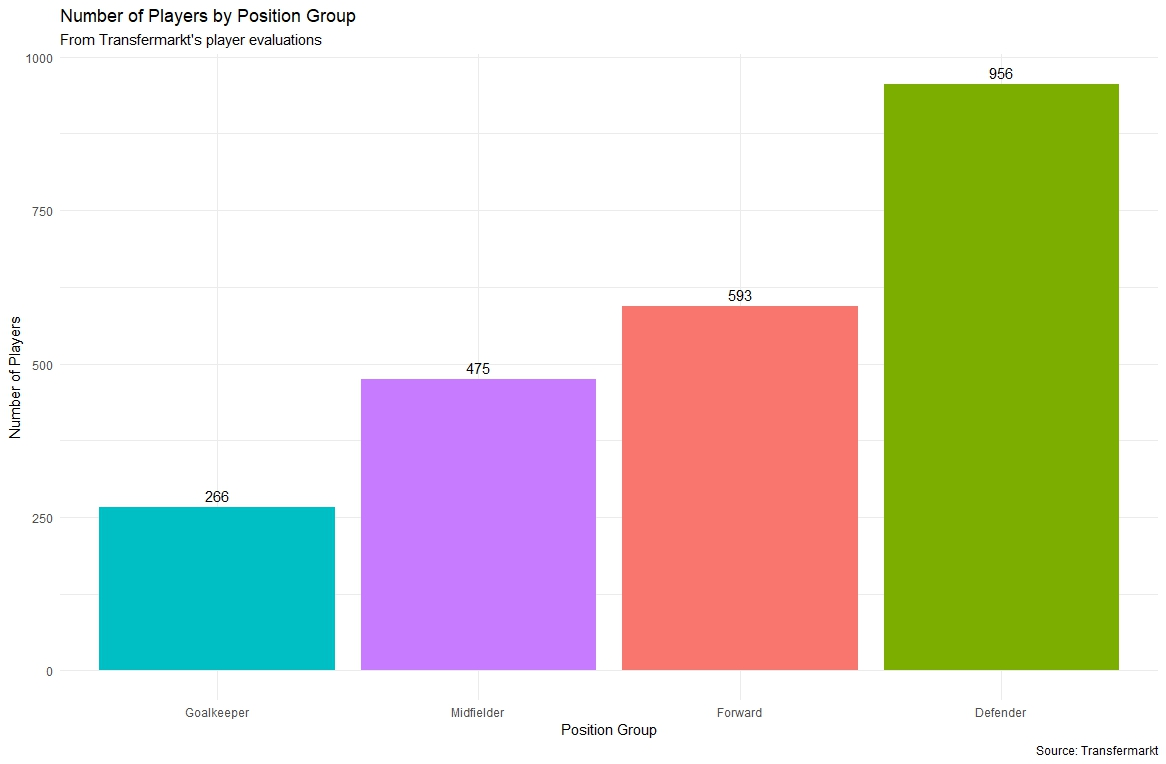
\includegraphics[width=0.95\textwidth, height=0.85\textheight, keepaspectratio]{pictures/Amount_Position_Groups.jpeg}
    \end{figure}
\end{frame}

% Slide 2
\begin{frame}
    \frametitle{Club Tier Distribution Across Leagues}
    \begin{figure}
        \centering
        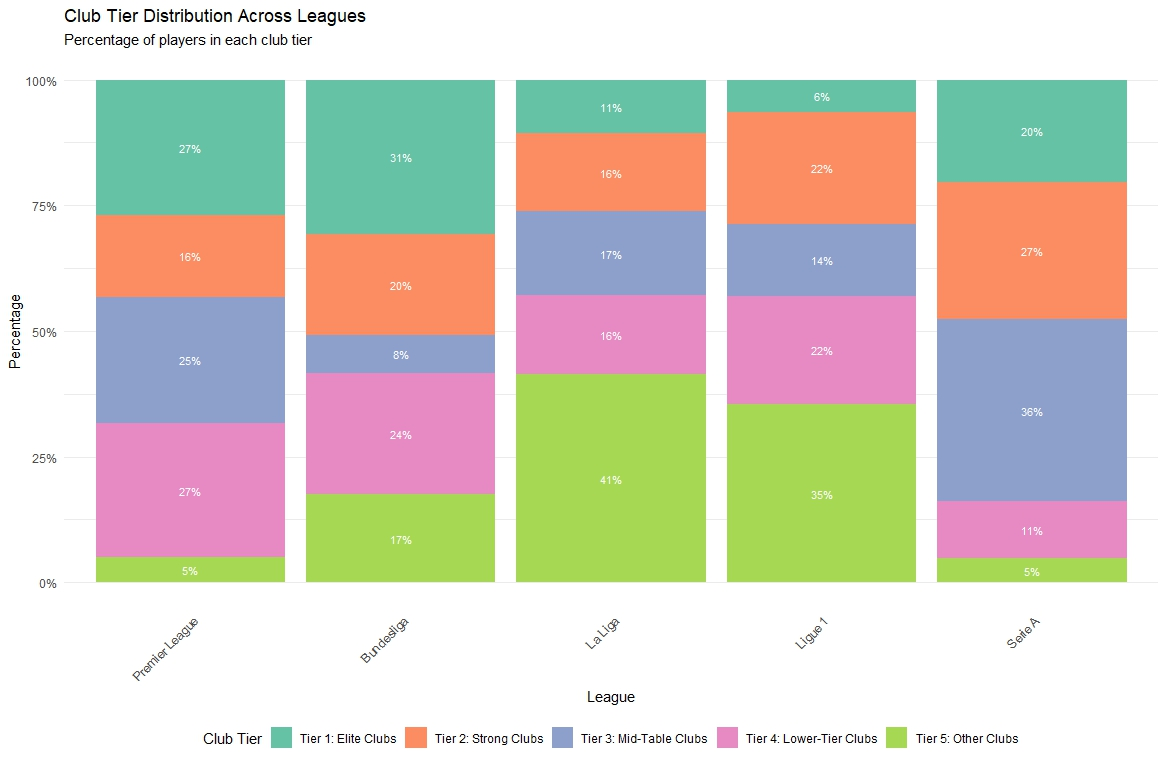
\includegraphics[width=0.95\textwidth, height=0.85\textheight, keepaspectratio]{pictures/Club_Distribution.jpeg}
    \end{figure}
\end{frame}
%~~~~~~~~~~~~~~~~~~~~~~~~~~~~~~~~~~~~~~~~~~~~~~~~
\section{Findings}
%~~~~~~~~~~~~~~~~~~~~~~~~~~~~~~~~~~~~~~~~~~~~~~~~
%~~~~~~~~~~~~~~~~~~~~~~~~~~~~~~~~~~~~~~~~~~~~~~~~
\subsection{Regression Findings}
%~~~~~~~~~~~~~~~~~~~~~~~~~~~~~~~~~~~~~~~~~~~~~~~~
%------------------------------------------------
%	NEW SLIDE
%------------------------------------------------
\begin{frame}[shrink=10]
    \frametitle{Regression Findings} 
    
    \begin{table}[ht]
        \scriptsize
        \centering
        \setlength{\tabcolsep}{3pt}
        \begin{tabular}{l|cccc}
            \hline
            \textbf{Variable} & \textbf{Forward} & \textbf{Midfielder} & \textbf{Defender} & \textbf{Goalkeeper} \\
            & $(N=593)$ & $(N=475)$ & $(N=956)$ & $(N=266)$ \\
            \hline
            Continent (Africa) & 0.041 & -0.104 & 0.176* & -0.079 \\
            Continent (S. America) & \cellcolor{yellow!30}0.425*** & \cellcolor{yellow!30}0.553*** & \cellcolor{yellow!30}0.378*** & \cellcolor{yellow!30}0.132 \\
            Age & 0.784*** & 1.103*** & 0.763*** & 0.842*** \\
            Age$^2$ & \cellcolor{red!20}-0.016*** & \cellcolor{red!20}-0.022*** & \cellcolor{red!20}-0.015*** & \cellcolor{red!20}-0.015*** \\
            Appearances & 0.022*** & 0.025*** & 0.024*** & 0.043*** \\
            Goal Contributions & 0.023*** & 0.014** & 0.009 & -- \\
            League (Bundesliga) & \cellcolor{blue!20}-1.004*** & \cellcolor{blue!20}-0.800*** & \cellcolor{blue!20}-1.024*** & \cellcolor{blue!20}-0.903*** \\
            League (La Liga) & -0.785*** & -0.609*** & -0.834*** & -0.210 \\
            League (Ligue 1) & -0.697*** & -0.349* & -0.890*** & -0.491* \\
            Club Tier (2) & -0.345** & -0.451*** & -0.652*** & -0.519* \\
            Club Tier (3) & -0.750*** & -0.989*** & -1.133*** & -0.962*** \\
            Club Tier (4) & -0.922*** & -1.110*** & -1.227*** & -0.866*** \\
            \hline
            Adjusted $R^2$ & \cellcolor{green!20}0.677 & \cellcolor{green!20}0.621 & \cellcolor{green!20}0.624 & \cellcolor{green!20}0.636 \\
            \hline
        \end{tabular}
        
        \vspace{1mm}
        {\footnotesize Significance: * $p<0.05$, ** $p<0.01$, *** $p<0.001$ \\
        Reference: Europe (Continent), Premier League (League), Tier 1 Elite Clubs (Club Tier) \\
        Interpretation: Percentage change in market value = $(e^{\beta} - 1) \times 100\%$ \\
        where $e$ is the base of the natural logarithm (approx. 2.718) and $\beta$ is the coefficient}
    \end{table}
\end{frame}
%------------------------------------------------
%	NEW SLIDE
%------------------------------------------------
%~~~~~~~~~~~~~~~~~~~~~~~~~~~~~~~~~~~~~~~~~~~~~~~~
\subsection{Peak Age}
%~~~~~~~~~~~~~~~~~~~~~~~~~~~~~~~~~~~~~~~~~~~~~~~~
% Slide 4
\begin{frame}
    \frametitle{Age-Value Relationship}
    \begin{figure}
        \centering
        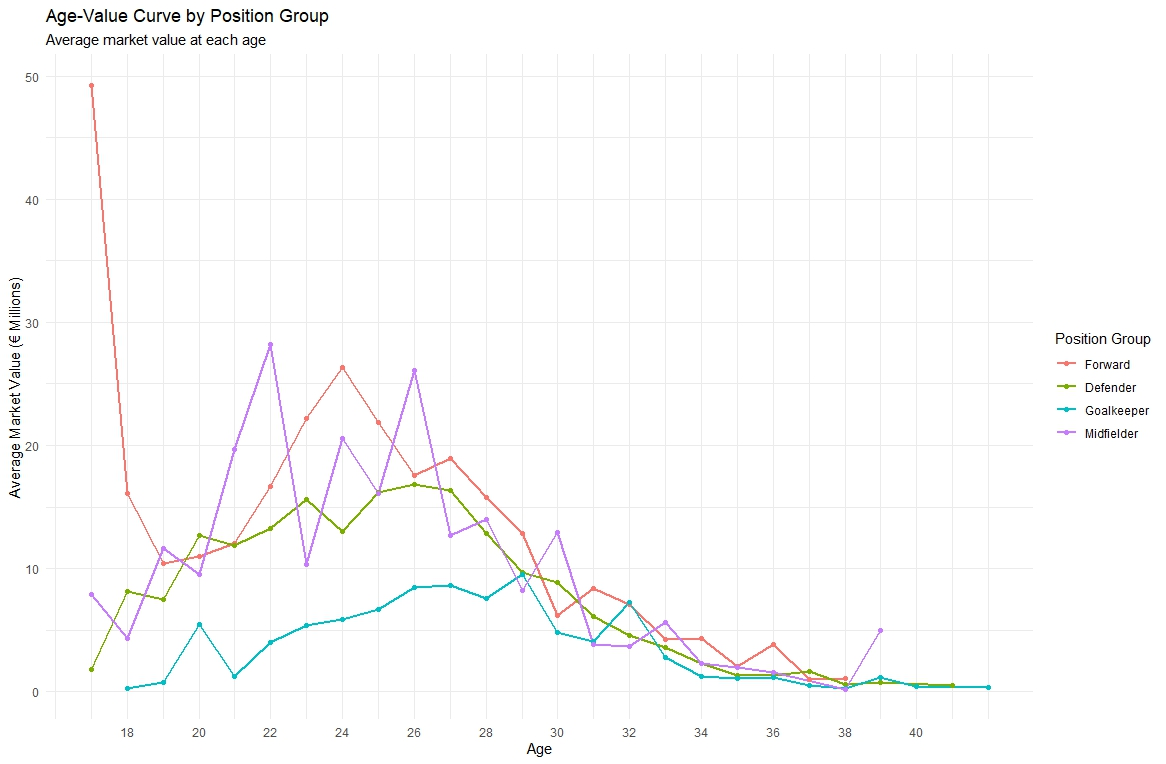
\includegraphics[width=0.95\textwidth, height=0.85\textheight, keepaspectratio]{pictures/Age_Value.jpeg}
    \end{figure}
\end{frame}


\begin{frame}
    \frametitle{Peak Market Value Age by Position} 
    
    \begin{center}
        \Large
        \textbf{Peak Age (Years)}
        
        \vspace{1cm}
        \begin{tabular}{lc}
            \hline
            \textbf{Position} & \textbf{Peak Age} \\
            \hline
            Forwards & 24.7 \\
            Midfielders & 25.5 \\
            Defenders & 24.7 \\
            Goalkeepers & 28.3 \\
            \hline
        \end{tabular}
        
        \normalsize
        Calculated as: $Peak Age = -\frac{\beta_{Age}}{2 \times \beta_{Age^2}}$
    \end{center}
\end{frame}
%~~~~~~~~~~~~~~~~~~~~~~~~~~~~~~~~~~~~~~~~~~~~~~~~
\section{Conclusion}
%~~~~~~~~~~~~~~~~~~~~~~~~~~~~~~~~~~~~~~~~~~~~~~~~
%~~~~~~~~~~~~~~~~~~~~~~~~~~~~~~~~~~~~~~~~~~~~~~~~
\subsection*{Conclusion}
%~~~~~~~~~~~~~~~~~~~~~~~~~~~~~~~~~~~~~~~~~~~~~~~~
\begin{frame}[shrink=15]
    \frametitle{Conclusion}
    
    \begin{itemize}\setlength{\itemsep}{0pt}
    
      \item Why does this matter?
      \begin{itemize}\setlength{\itemsep}{0pt}
        \item There is a large amount of money spent in worldwide football. These values impact millions around the world.         
        \item The $R^2$ values around 0.62-0.68 indicate these factors collectively explain roughly two-thirds of the variation in player market values. 
        \item The subjective factors used by Transfermarkt are explainable with measureable factors. 
      \end{itemize}
      \vspace{0.2cm}
    \end{itemize}
\end{frame}
%~~~~~~~~~~~~~~~~~~~~~~~~~~~~~~~~~~~~~~~~~~~~~~~~
\section{References}
%~~~~~~~~~~~~~~~~~~~~~~~~~~~~~~~~~~~~~~~~~~~~~~~~
\begin{frame}
\frametitle{References}
\bibliographystyle{apalike}
\bibliography{references}
\end{frame}

%================================================
%	END DOCUMENT 
%================================================
\end{document}
